\begin{tikzpicture}
  \draw[thin,->] (-pi/2-0.1,0)--(5*pi/2+0.1,0) node[right] {$\omega t$};
  \draw[thin,dashed] (-pi/2-0.1,0.5)--(5*pi/2+0.1,0.5);
  \draw[domain=-pi/2:pi/2]
  plot (\x, {cos(\x r)});
  \draw[domain=pi/2:3*pi/2]
  plot(\x, {cos((\x-pi) r)});
  \draw[domain=3*pi/2:5*pi/2]
  plot (\x, {cos(\x r)});
  %  \draw[domain=3*pi/2:2*pi]
  %  plot(\x, {-cos(\x r)});
  \draw[thin,<->] (0,0.5)--(0,1);
  \draw[thin,<-] (0,0.75)--(1,1.3) node[right]{амлитуда положительной полуволны};
  \draw[thin,<->] (pi/2,0)--(pi/2,0.5);
  \draw[thin,<-] (pi/2,0.25)--(pi/2+1,-0.3) node[right]{амлитуда отрицательной полуволны};
\end{tikzpicture}

Можно ли считать полную амплитуду удвоением амлитуды нижней полуволны. Точного
расчёта пульсаций тока не существует.

Размах колебаний $(A_+ + A_-)$.

Зачем ограничивать пульсации тока. Каким образом выбирать ограничения. Ограничивают,
потому что потери на $R$ чем меньше тем лучше. Но ноль не может быть. Граница прерывистого
режима плохо. Чем меньше граница тем лучше.

Хороший критерий был -- электропривод постоянного тока. Но коллектор -- слабое место.
Коллектор--пластины--искрение, меняется магнитный поток. Нужно постараться, чтобы
тока в этот момент не было. ЭДС движения... Сумма ЭДС должна быть равна 0.
$I_\textcyrillic{якоря максимум}$ -- ограничивают.

$n_\textcyrillic{оборотов}$ -- $\frac{\partial i}{\partial t}$ тем больше искрение.
Переменная составляющая  тока. Добавил пульсации -- возникло искрение
$L\frac{\partial i}{\partial t}$ -- от переменной составляющей. А от частоты зависит
переменная составляющая? Принято считать, что не зависит, 2\% от номинального
для крупных машин. Станина -- литая сталь, поковка, литьё. Наборные пластины -- дорого.
Если поток добавочных полюсов должен компенсировать $I_\textcyrillic{якоря}$
Якорь шихтованный -- нет намагничивающих токов и поток не запаздывает, а в станине
эти эффекты ограничивают 2\%
Станина тоже из стали: из шихтованной стали 20\% пульсации

$
{\scriptstyle \Delta} I = I^2_\textcyrillic{ном} R
$
несколько процентов 3-2\%. КПД 96.5 - 3,4\% -- потери стали,меди,механические.

Добавилась пульсация 5\%
$$
I = \sqrt{I^2_\textcyrillic{пост} + I^2_\textcyrillic{перем}} R
$$

Выражение граничного тока:

$$
I_{d\textcyrillic{гран}} = \frac{E_{d0}}{\omega L}\left[1-\frac{\pi}{m}\,ctg \frac{\pi}{m}
\right]
\,sin\,\alpha
$$
где, $\omega$ -- питающей сети. $\omega_\textcyrillic{сети} =2\pi f_\textcyrillic{сети}$
Максимум при  $\alpha=90^\circ$, очевидно, зависит от числа фаз.

Это выражение даст эллипс

\begin{tikzpicture}
  %ellipse elipse
  \draw[domain=0:0.7, help lines,dotted, smooth]
  plot (\x,{sqrt(1-\x*\x/0.49)});
  \draw[domain=0:0.7, help lines,dotted, smooth]
  plot (\x,{-sqrt(1-\x*\x/0.49)});
  \draw[thin] (0.2,0) -- (0.2,{sqrt(1-0.2*0.2/0.49)}) --++ (2,-0.3);
  \draw[thin] (0.5,0) -- (0.5,{sqrt(1-0.5*0.5/0.49)}) --++ (2,-0.3);
\end{tikzpicture}

\subsection{Энергетические характеристики тиристорных преобразователей}

КПД $\eta = f(U_d)$, при $I_d=const$. Зависимость от напряжения и тока, $\alpha$ -- управления.

Электрические машины:
\begin{itemize}
\item постоянного тока(генераторы,моторы))
\item синхронные
\item асинхронные
\item трансформаторы 
\end{itemize}

Напряжение сети $=const$, от $cos\,\phi$

В электрических машинах $\displaystyle \eta = f(\frac{I}{I_\textcyrillic{ном}})$ или
$\displaystyle f(\frac{S}{S_\textcyrillic{ном}})$ или
$\displaystyle f(\frac{P}{P_\textcyrillic{ном}})$, $cos\,\phi$

У синхронных генераторов зависимость от $\phi$ нагрузки.

Когда я меняю напряжение интересует что будет с $cos\,\phi$

КМ($\lambda$) --коэффициент мощности, есть отношение активной мощности к полной.

$$
\textcyrillic{КПД} = \frac{P_\textcyrillic{вых}}{P_\textcyrillic{входа}}
$$

$$
\lambda = \frac{P}{S}
$$
где, $P$ -- активная мощность, $S$ -- полная мощность.

$
\textcyrillic{Коэффициэнт мощности} = cos\,\phi
$ -- неверно в общем случае. Так можно говорить, если напряжение
симметрично, синусоидально, и одной частоты. В нашем случае разные частоты.

Допущение: сеть симметрична и синусоидальна.

$$
\lambda = \frac{S_{(1)}}{S}\cdot\frac{P}{S_{(1)}}
$$

$S$ -- полная мощность $U\cdot I$ формальное произведение.

$S_{(1)} = U_{(1)}\cdot I_{(1)}$ -- если однофазная система.
$$
S =\underbrace{U_\textcyrillic{средне квадратичное}}_
{\textcyrillic{по допущению }U_1}\cdot I_\textcyrillic{средне квадратичное}
$$
А ток -- это наш ток и мы знаем, что он несинусоидальный. Если включу
на активное сопротивление последовательно 100V и 100V, получу 200V.
А если включить на активно-индуктивную нагрузку.
У нас было 50Гц, А в токе разные частоты. Другие частоты в токе несут ли
активную и реактивну мощность? Несут токи одинаковой частоты
$U(\omega)\cdot I(\omega)$ -- одинаковой частоты.
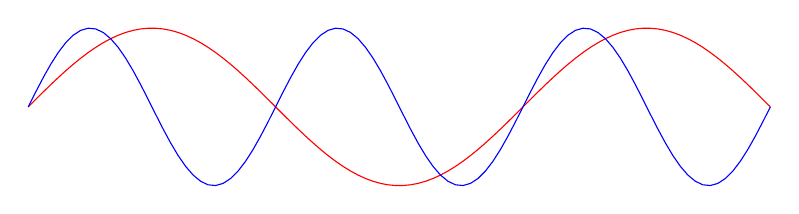
\begin{tikzpicture}
  \draw[domain=0:3*pi,samples=100,red]
  plot(\x, {sin(\x r)});
  \draw[domain=0:3*pi,samples=100,blue]
  plot(\x,{sin((2*\x) r)});
\end{tikzpicture}

Есть колебательная мощность. Это реактивная? нет

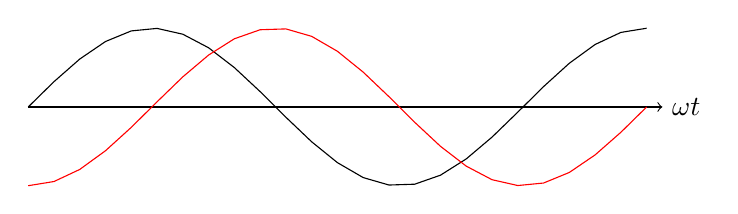
\begin{tikzpicture}
  \draw[thin,->] (0,0)--(2*pi+pi/2+0.2,0) node[right] {$\omega t$};
  \draw[domain=0:2*pi+pi/2]
  plot(\x,{sin(\x r)});
  \draw[domain=0:2*pi+pi/2,red]
  plot(\x,{sin((\x-pi/2) r)});  
  \end{tikzpicture}

Знаки разные(в этом смысле похоже на предыдущий случай), но не совсем. <могу поставить <C> и
скомпенсировать>

$$
\begin{array}{cccc}
  P&[\textcyrillic{вт}]&=&UI_\textcyrillic{актив}\\
  Q&[\textcyrillic{вар}]&=&UI_\textcyrillic{реактив}\\
  S&[\textcyrillic{ВА}]&=&{\displaystyle S=\sqrt{P^2+Q^2}}
  \end{array}
$$
Эти соотношения для одинаковых частот.

Если частоты разные, то это мощность искажения
$$
\lambda = \frac{S_1}{S}\frac{P}{S_1} = \nu\,cos\,\phi
$$,
где $S_1 = U_1\cdot I_1$

Нелинейные нагрузки искажают форму тока, портят стандарты, требуют принятия мер для качетва напряжения.
Несинусоидальность не больше стольки-то \%.

Пренебрегаем влиянием внешних.

$$
\eta = \frac{P_\textcyrillic{вых}}{P_\textcyrillic{вх}}
$$
$$
\lambda = \frac{S_1}{S}\frac{P}{S_1} = \nu\,cos\,\phi
$$

Наша специальность самая энернгетическая.

$$
Р\textcyrillic{вых} = U_dI_d
$$

$$
Р\textcyrillic{вх} = Р\textcyrillic{вых} + {\scriptstyle \Delta}P_\Sigma
$$,
где $P_\Sigma$ -- потери, то что преобразовалось в тепло, электромагнитную волну, звук, свет.

Представим, что мы регулируем напряжение.

$$
\eta = \textcyrillic{КПД} = \frac{U_d\,I_d}{U_d\,I_d + {\scriptstyle \Delta}P_\Sigma}
$$

${\scriptstyle \Delta}P_\Sigma $ на активных элементах:
  $I_d^2\,r_{\Sigma\textcyrillic{эквив}} +...+I_d\,k_0U_0 + {\scriptstyle \Delta}P_{xx}$,
  где $k_0U_0$ может быть несколько вентилей. Ток в вентилях меняется пропорционально $I_d$,
  $I_\phi$ -- в обмотке трансформатора. $I_\phi\div I_d$ (ток в обмотке трансформатора пропорционален
  $I_d$, в два раза увеличилось $I_\phi$, значит в два раза увеличилось $I_d$, т.е. есть
  составлающая пропорциональная $I_d$)

  А если выключено, потери не зависят от $I_d$ (система управления, лампочки)

  $$
  = aI^2_d + bI^1_d + cI^0_d
  $$

  $$
  \eta = (\textcyrillic{добавил и вычел } \pm {\scriptstyle \Delta}P_\Sigma) =
  1 - \frac{{\scriptstyle \Delta}P_\Sigma}{U_dI_d +{\scriptstyle \Delta}P_\Sigma} =
\label{eta}
  $$
Выражение(\ref{eta}) меньше единицы когда и $U_d$ и $I_d$ одного знака. $I_d>0$ всегда больше нуля.
значит $0<U_d<0$ (может быть и больше и меньше нуля)

$$
= 1 - \frac{\displaystyle \frac{{\scriptstyle \Delta}P_\Sigma}{U_d\,I_d}}
{\displaystyle 1\;+\;\frac{{\scriptstyle \Delta}P_\Sigma}{U_d\,I_d}}
$$

Сейчас будем рассматривать $I_d=const$ при бесконечном увеличении $U_d$ $\eta\rightarrow1$
Но $U_d$ не больше чем $U_{d\;max}$

\begin{tikzpicture}
  \begin{scope}[scale=5]
    \draw[thin,->] (-1.2,0)--(1.2,0) node[right]{$\frac{U}{E_{d0}}$};
    \draw[thin,->] (0,-0.1)--(0,1.2) node[left]{$\eta$};
    \draw[thin,dotted] (-1,0)--(-1,1)--(1,1)--(1,0);
    \draw[thin,dotted] (-1.2,1) -- (-1,1);
    \draw[thin,dotted] (1,1) -- (1.3,1);
  \draw[domain=0.001:0.8]
  plot(\x, {1-(1/\x)/(10+(1/\x))});
  \draw[domain=0.8:1.3,dashed]
  plot(\x, {1-(1/\x)/(10+(1/\x))});
  \draw[domain=-0.8:-0.1]
  plot(\x, {1+(1/\x)/10});
  \draw[domain=-1.2:-0.8,dashed]
  plot(\x, {1+(1/\x)/10});
  %
  \draw[thin,dashed]  (0.8, {1-(1/0.8)/(10+(1/0.8))})-- (0.8,0) node[below]
       {$\frac{U_{d\,max}}{E_{d0}}$};
       \draw[thin,dashed]  (-0.8, {1+(1/(-0.8))/10}) -- (-0.8,0) node[below]
       {$\frac{U_{d\,max}}{E_{d0}}$};
  
  %если ток вырос
  \draw[domain=0.001:0.8,dashed]
  plot(\x, {1-(1/\x)/(7+(1/\x))});
  \draw[domain=-0.8:-0.125,dashed]
  plot(\x, {1+(1/\x)/8});
  %
  \draw[thin,<-] (-0.1,0)--(0.3,-0.3) node[below]{$U_d=-\frac{{\scriptstyle \Delta}P_\Sigma}{I_d}$};  
  \draw[thin,<-] (-0.125,0) -- (-0.4,-0.3) node[below]{если ток вырос};

  \draw[thin,<-] (0.7,{1-(1/0.7)/(10+(1/0.7))}) -- (0.9,0.7) node[right] {$I_d=const$};
  \draw[thin,<-] (-0.7,{1+(1/(-0.7))/10}) -- (-0.9,0.7) node[left] {$I_d=const$};
  \draw[thin,<-] (0.6, {1-(1/0.6)/(7+(1/0.7))}) -- (0.6,0.5) node[right] {$I_{d2}>I_{d1}$};
  %  \draw[thin,<-]]
  \end{scope}
  \end{tikzpicture}


$P_\textcyrillic{вых}$. При отрицательном $\eta$ поменялись местами выход и вход.
То, что было $\eta_\textcyrillic{выпрямителя}$ при $(U_d>0)$ стало
при $U_d<0$

$$
\eta_\textcyrillic{инвертора} = \frac{U_d\,I_d+{\scriptstyle \Delta}P_\Sigma}
    {U_d\,I_d} = 1 +\hspace{-0.8cm}
    \underbrace{\frac{{\scriptstyle \Delta}P_\Sigma}{U_d\,I_d}}_
               {\begin{array}{c}\textcyrillic{отрицательно}\\
                   \textcyrillic{эта дробь}\\
                   \textcyrillic{станет равна -1}\end{array}}
               $$
при $\displaystyle u_d = -\frac{{\scriptstyle \Delta}P_\Sigma}{I_d}$
-- КПД упадёт до 0 и обратно пропорционально току.

$$
{\scriptstyle \Delta}P_\Sigma = \frac{a\,I_d^2}{I_d} 
$$

$\eta_\textcyrillic{граничное} =0!$ при $U_d>0$

$\eta_\textcyrillic{граничное}$ при $\displaystyle U_d< U_{d_\textcyrillic{граничное}} =
-\frac{{\scriptstyle \Delta}P_\Sigma}{I_d}$

Осталось понять чему равен $\eta$ при $U_{d_\textcyrillic{граничное}}<U_d<0$:

\underline{$\eta$ по определению} равен нулю потому что $P_\textcyrillic{вых}$ =0.

\subsection{Энергетические реки:}

\begin{tikzpicture}
  \draw[thick,help lines] (0,3)--(5,3);
  \draw[thick,help lines] (0,0)--(2,0)arc(90:0:1);
  \draw[thick,help lines] (2,0.8)arc(90:0:1.8);
  \draw[thick,help lines] (2,0.8)--(5,0.8);
  \draw (-0.8,1.3) node[left] {сеть};
  \draw[<-,double] (0.8,1.7)--(0.3,1.7) node[left]{$P_\textcyrillic{вх}$};
  \draw[->,double] (4.2,1.7)--(4.7,1.7) node[right]{$P_\textcyrillic{вых}$};
  \draw[->,double] (3.15,-0.3) arc(40:0:1.1) node[below]
       {${\scriptstyle \Delta} P_\Sigma$};
   \draw (5.8,1.3) node[right] {нагрузка};
\end{tikzpicture}


\begin{tikzpicture}
  \draw[thick,help lines] (0,3)--(5,3);
  \draw[thick,help lines] (5,0)--(3,0)arc(90:180:1);
  \draw[thick,help lines] (3,0.8)arc(90:180:1.8);
  \draw[thick,help lines] (3,0.8)--(0,0.8);
  \draw (-0.8,1.3) node[left] {сеть};
  \draw (5.8,1.3) node[right] {нагрузка};
  \draw[->,double] (4,0.4)--(3,0.4)arc(90:180:1.4) node[below]
  {${\scriptstyle \Delta} P_\Sigma$};
  \draw[<->,thin] (0.2,3)--(0.2,0.8) node[midway,right]
       {$P_\textcyrillic{сети}=P_\textcyrillic{вых}$};
  \draw[<->,thin] (4.8,3)--(4.8,0) node[midway,right]
       {$P_\textcyrillic{вх}$};
  \draw[thick,help lines] (4.6,1)--(3.6,1);
  \draw[thin,<-] (4.4,1)--(4.4,-0.6) node[below]
       {$\begin{array}{c}\textcyrillic{сокращается }U_d\,I_d,\\
         \textcyrillic{а потери неизменны}\end{array}$};
\end{tikzpicture}  


\begin{tikzpicture}
    \draw[thin,->] (-1.2,0)--(1.2,0);% node[right]{$\frac{U}{E_{d0}}$};
    \draw[thin,->] (0,-0.1)--(0,1.1);
    \draw[domain=-0.8:-0.1]
    plot(\x, {1+(1/\x)/10});
    \draw[thin,<-] (-0.1,-0.05)-- (-0.4,-0.5) node[below]
    {Нагрузка едва покрывает потери};
\end{tikzpicture}    
%--Нагрузка едва покрывает потери.

Нагрузка отдает, а до сети ничего не доходит.

\begin{tikzpicture}
  \draw[thick,help lines] (0,0.8)--(5,0.8);
  \draw[thick,help lines] (0,0)--(1,0)arc(90:0:1);
  \draw[thick,help lines] (5,0)--(4,0)arc(90:180:1);
  \draw[->,double] (0.2,0.35)--(0.95,0.35)arc(90:0:1.35)
  node[below] {${\scriptstyle \Delta}P_\Sigma\textcyrillic{ потери}$};
  \draw[->,double] (4.8,0.35)--(4.05,0.35)arc(90:180:1.35);
  
\end{tikzpicture}
Нагрузка не выпрямительный режим, но и не инверторный.
Получают только потери.

А если $I_d$ изменится: $I_d$ вырос в два раза, числитель вырастет в два раза,
но и ${\scriptstyle \Delta}P_\Sigma$ тоже вырастет. Всё зависит от
коэффициента(-тов).

Реально, КПД упадт.

слева, при большом токе вырастет $\gamma$

\subsection{Коэффициент мощности}
$\nu$ -- коэффициэнт искажения $cos\,\phi$ -- коэффиниент угла сдвига тока,
численно равен коэф мощности, когда напряжение и ток синусоидальны.

$$
cos\,\phi = \frac{P}{S}
$$

$S$ всегда положительна, $P$ бывает и положительна и отрицательна.
$Q>0$ -- индуктивность, так принято. Преобладают нагрузки, которые
потребляют положительную реактивную мощность.
В воздушной линии $C\sim\frac{S}{d}$
В кабельных линиях -- емкости.

$C$ генерирует в сеть реактивную мощность.

$\phi$ положительный, когда ток отстает от напряжения.

$sin\,\phi<0 \Rightarrow Q<0$

Cos может быть и положительным и отрицательным.

$$
\frac{P}{S} = |I|\cdot|U|\cdot cos\,\phi
$$

$cos\,\phi=-0.5$ Инвертор работает с углом $\sim 60^\circ$.

Реактивная мощность не передаёт балластную мощность. Из-за реактивных токов
приходится увеличивать мощность <приборов,трансформаторов>

Ток, который создаёт магнитное поле

$$
L=\frac{\Phi}{i}
$$

У синхронных машин магнитное поле создаётся обмоткой возбуждения.
У аснхронных двигателей создаётся реактивным током.

$\alpha$ сдвинул на $90^\circ$ -- я принудительно сдвинул начало генерации тока.

\begin{tikzpicture}
  % оси
  \draw[thin,->] (-pi/2,0)--(2*pi,0) node[right]{$\omega t$};
  \draw[thin,->] (-pi/2,-0.1)--(-pi/2,1.2) node[left] {$U$};
  \draw[thin,->] (-pi/2,-1.5)--(2*pi,-1.5) node[right]{$\omega t$};
  \draw[thin,->] (-pi/2,-1.6)--(-pi/2,-0.4) node[left] {$I$};
  %
  \draw[domain=-pi/2:pi/2,help lines,smooth]
  plot(\x, {cos(\x r)});
  \draw[domain=pi/6:7*pi/6,help lines,smooth]
  plot(\x, {cos((\x-2*pi/3) r)});
  \draw[domain=5*pi/6:11*pi/6,help lines,smooth]
  plot(\x, {cos((\x-4*pi/3) r)});
  % 
  \draw[thin,red,domain=-pi/3+0.3:-pi/3+2*pi/3+0.3]
  plot(\x, {cos(\x r)+0.05})
  |- (pi/3+0.3, {cos((pi/3+0.3-2*pi/3) r)+0.05});
  \draw[thin,red,domain=-pi/3+2*pi/3+0.3:-pi/3+4*pi/3+0.3]
  plot(\x, {cos((\x-2*pi/3) r)+0.05})
  |- (-pi/3+4*pi/3+0.3, {cos((-pi/3+4*pi/3+0.3-4*pi/3) r)+0.05});
  \draw[thin,red,domain=-pi/3+4*pi/3+0.3:-pi/3+6*pi/3+0.3]
  plot(\x, {cos((\x-4*pi/3) r)+0.05});
  %
  \draw[help lines,smooth] (-pi/2,-1.3)--(-pi/3,-1.3)--(-pi/3,-0.8)--(pi/3,-0.8)
  --(pi/3,-1.3)--(pi/2,-1.3);
  \draw[help lines,smooth] (pi/6,-0.6) node[right]{$I(\alpha=0)$};
  \draw[help lines,smooth,red](-pi/2+0.3,-1.4)--(-pi/3+0.3,-1.4)--
  (-pi/3+0.3,-0.9)--(pi/3+0.3,-0.9)--(pi/3+0.3,-1.4)--(pi/2+0.3,-1.4);
  \draw[red] (pi/2,-1.2)node[right]{$I(\alpha>0)$};
  %
  \draw[thin] (0,-0.8) -- (0,-2);
  \draw[thin] (0.3,-0.9) -- (0.3,-2);
  \draw[thin,->] (-0.3,-1.9)--(-0,-1.9);
  \draw[thin,<-] (0.3,-1.9)--(0.8,-1.9) node[right]
       {$\phi\approx\alpha\textcyrillic{ в первом приближении}$};
  \draw[thin,<-] (-0,-2.1)--(-0.3,-2.1) node[left]{$\alpha$};
  \draw[thin,<-] (0.3,-2.1)--(0.5,-2.1);
\end{tikzpicture}

$\alpha=0$ -- фаза тока совпадает с фaзой напряжения. $\phi = \alpha$ в
первом приближении.

Насколько сдвинулись гармоники тока? Но это никак не связано с энергией!

$I_d=const$ будем рассматривать для всех энергетических характеристик.

$$
P=U_d\,I_d\;\; \xcancel{(+{\scriptstyle \Delta}P_\Sigma)}
$$
равенство буду считать хотя бы примерно(пока не буду считать потери)

Поддерживая $I_d=const$ $S$ будет оставаться неизменной.
$S_1 \cong const$, потому что $I_d \cong const$

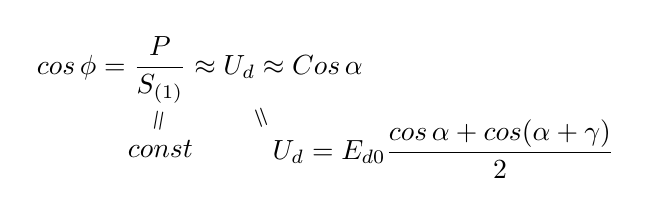
\begin{tikzpicture}
  \draw (0,1) node {$\displaystyle cos\,\phi = \frac{P}{S_{(1)}} \approx U_d \approx Cos\,\alpha$};
  \draw (-0.5,0.35) node[rotate=80] {=};
  \draw (-0.5, 0) node{$const$};
  \draw (0.8,0.4) node[rotate=110] {=};
  \draw (0.8,0) node[right]
   {$\displaystyle U_d=E_{d0}\frac{cos\,\alpha + cos(\alpha+\gamma)}{2}$};
\end{tikzpicture}

При $\alpha=0\;\gamma=0$ $U_d=E_{d0}$

Чисто активная мощность, значит ...

При $\alpha=0\;\gamma=0$ $U_d=E_{d0}$, $P=S_1$

$P\Bigl|_{\scriptstyle \begin{array}{c}\scriptstyle{\alpha=0}\\
    \scriptstyle{\gamma=0}\end{array}} = S_1 = E_{d0}I_d$

при $P$, которое я регулирую

$$
\frac{P}{S} = \frac{E_d\,I_d \frac{cos\,\alpha + cos(\alpha+\gamma)}{2}}{E_d\,Id}
$$

отсюда
$$
cos\,\phi = \frac{cos\,\alpha + cos(\alpha + \gamma)}{2}
$$
достаточно точно, угол $\phi$ пропорционален $\alpha$.
